% Technical document (English).
% Build:  cd reports/technical_document && latexmk -pdf report_en.tex     (or: pdflatex report_en.tex, twice)
% Figures are produced by ../make_figures.py (the _en versions) from the logged runs in docs/data/.
\documentclass[11pt,a4paper]{article}

\usepackage[T1]{fontenc}
\usepackage[utf8]{inputenc}
\usepackage{lmodern}
\usepackage[margin=2.5cm]{geometry}
\usepackage{amsmath,amssymb}
\usepackage{graphicx}
\usepackage{booktabs}
\usepackage{array}
\usepackage{float}
\usepackage{caption}
\usepackage[hidelinks]{hyperref}
\usepackage{url}

\graphicspath{{../figures/}{../../docs/}}
\renewcommand{\arraystretch}{1.15}
\captionsetup{font=small,labelfont=bf}
\setlength{\parskip}{4pt}
\setlength{\parindent}{0pt}
\emergencystretch=3em
\newcommand{\code}[1]{\texttt{\small #1}}

\title{\textbf{Technical and System Design Document}\\[4pt]
\large Four-wheel omnidirectional robot controlled by two-handed gestures\\
\normalsize AI-Powered Omni Robot project, version 2}
\author{Tai Nguyen Anh}
\date{November 2026}

\begin{document}
\maketitle
\tableofcontents
\newpage

%====================================================================
\section{System Overview}
\subsection{Problem and Design Goals}
A differential-drive robot cannot slide sideways, whereas an omnidirectional robot with four wheels in a $45^\circ$ X arrangement moves in any direction on the plane with three independent velocities: forward ($v_x$), sideways ($v_y$) and rotation ($\omega$). Gesture interfaces usually handle only driving, while changing mode, setting speed or pressing the emergency stop still needs a mouse or keyboard.

The project does both with a single laptop camera:
\begin{itemize}
  \item The \textbf{dominant hand} controls the web interface: it moves the cursor, holds still to click, and raises the middle finger to press or drag the virtual joystick and the sliders.
  \item The \textbf{non-dominant hand} drives the robot with 8 pointing directions and a V sign for rotation. In Manual mode (virtual joystick, keyboard) any single hand is enough to operate the interface.
\end{itemize}
The robot hardware is an ESP32 with two L298N H-bridges and four GM25-370 motors with encoders. The ESP32 creates its own Wi-Fi network and receives commands over UDP.

\subsection{Targets and Measured Results}
The targets in Table~\ref{tab:spec} were set by the team as reference marks, not as external requirements. The results column comes from the measurements in Section~\ref{sec:verify}.

\begin{table}[H]
\caption{Targets and measured results.}
\label{tab:spec}
\centering\small
\begin{tabular}{p{4.6cm}p{2.3cm}p{5.2cm}}
\toprule
Item & Target & Measured result \\
\midrule
Camera + hand detection loop rate & $\ge 25$ fps & 29.9 fps without hands (isolated benchmark); 18.0--25.5 fps in server sessions, inference 45.5--55.5 ms with one hand \\
UDP round-trip time (RTT) & $<50$ ms (median) & median 6.6--8.1 ms; P95 16.1--26.1 ms \\
Per-wheel speed tracking error (mean) & $<5.0\,\%$ & 1.5--3.2\,\% of full speed; P95 4.4--7.4\,\% \\
Body velocity deviation from command & $<5.0\,\%$ & 0.1--2.5\,\% on the main axis; other axes $\le 0.004$ \\
From confirmed gesture to wheel at 50\\,\\% & $<400$ ms & median 427 ms (321--496), 15 events, measured from the camera frame (not met); earlier runs 257--260 ms, measured from the logged gesture \\
Fail-safe stop on lost command & $<500$ ms & ESP32 300 ms; laptop 400 ms; jam protection 700 ms \\
\bottomrule
\end{tabular}
\end{table}
Note: the 29.9 fps and 18.5 ms inference were measured on 12 November 2026 over 359 consecutive frames; the gesture-to-wheel latency includes the deliberate acceleration limit (Section~\ref{sec:control}) and excludes the 4 frames (about 133 ms) needed to confirm a gesture.

\subsection{Overall Architecture}
The system has two parts connected by a Wi-Fi network created by the ESP32 itself (SSID \code{omni-robot}, fixed IP \code{192.168.4.1}, UDP port 4210), with no Internet needed (Fig.~\ref{fig:arch}).

\begin{itemize}
  \item \textbf{Laptop (host)}: \code{ai/camera.py} reads MJPG $1280\times720$ images at 30 fps in a separate thread (detection runs on a 640-px-wide copy) that keeps only the newest frame. MediaPipe HandLandmarker returns 21 landmarks for up to 2 hands. \code{RoleAssigner} and \code{split\_roles()} send the dominant hand to the cursor controller (\code{ai/ui/cursor.py}) and the non-dominant hand to the driving gesture classifier (\code{ai/drive/}). The 20 Hz \code{control\_loop()} selects the command according to the mode, limits its acceleration, and sends it by UDP through \code{RobotLink}.
  \item \textbf{ESP32 (edge)}: receives the command packet, checks the single-owner lock and the 300 ms timeout, computes inverse kinematics, runs 4 speed controllers every 10 ms, outputs PWM to the two L298N modules, and returns an acknowledgement with the target speed, measured speed and PWM of the 4 wheels.
\end{itemize}

\begin{figure}[H]
  \centering
  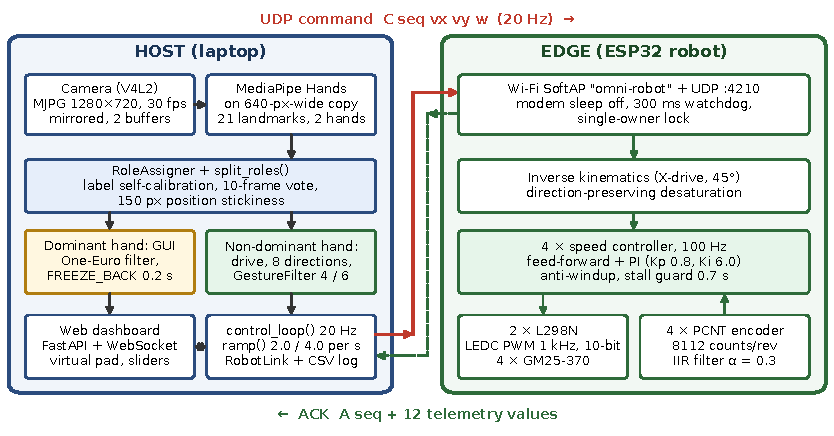
\includegraphics[width=\textwidth]{fig_arch_en.pdf}
  \caption{Host--edge architecture. Solid red: UDP command; dashed green: acknowledgement with wheel telemetry.}
  \label{fig:arch}
\end{figure}

%====================================================================
\section{Mechanics and Kinematics}
\subsection{Configuration}
The four omni wheels sit at the four corners with their main rolling axis tilted $\pm45^\circ$ from the body's longitudinal axis (X arrangement), directly on the output shafts of four $1{:}78$ geared motors. The code uses the ROS convention: $+x$ forward, $+y$ to the left, and $+\omega$ counter-clockwise seen from above (Fig.~\ref{fig:kin}). Wheel indices: 0 front-left (tt), 1 front-right (tp), 2 rear-left (st), 3 rear-right (sp). Positive wheel speed is the direction that moves the robot forward.

\begin{figure}[H]
  \centering
  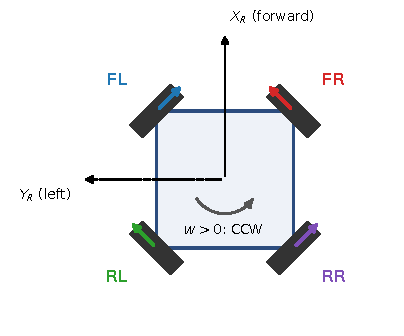
\includegraphics[width=0.5\textwidth]{fig_kin_en.pdf}
  \caption{X-configuration geometry and the thrust direction of each wheel when rolling forward.}
  \label{fig:kin}
\end{figure}

\subsection{Inverse Kinematics and Direction Preservation}
In the firmware (\code{firmware/src/kinematics.h}) velocities are normalized to $[-1,1]$, with 1.0 corresponding to \code{MAX\_CPS} $=4300$ counts/s (about 31.8 rpm). With $\mathbf u=[v_x,v_y,\omega]^\top$:
\begin{equation}
\begin{bmatrix}r'_{tt}\\r'_{tp}\\r'_{st}\\r'_{sp}\end{bmatrix}=
\begin{bmatrix}1&-1&-1\\1&1&1\\1&1&-1\\1&-1&1\end{bmatrix}\mathbf u,\qquad
r_i=\frac{r'_i}{m},\quad m=\max\bigl(1,\max_j|r'_j|\bigr).
\label{eq:ik}
\end{equation}
Dividing by the common factor $m$ keeps the ratio between the wheels when one exceeds 1.0, so the robot only slows down and does not change direction. Clipping each wheel separately would distort the ratio and make the robot drift.

\subsection{Forward Kinematics}
The columns of the matrix in (\ref{eq:ik}) are orthogonal with squared norm 4, so its pseudo-inverse is the transpose divided by 4. From the measured speeds $m_i$ of the 4 wheels, \code{tests/analyze\_drive\_log.py} recomputes the body velocity:
\begin{equation}
\begin{bmatrix}v_x\\v_y\\\omega\end{bmatrix}_{\text{odo}}=\frac14
\begin{bmatrix}1&1&1&1\\-1&1&1&-1\\-1&1&-1&1\end{bmatrix}
\begin{bmatrix}m_{tt}\\m_{tp}\\m_{st}\\m_{sp}\end{bmatrix}.
\label{eq:fk}
\end{equation}

%====================================================================
\section{Hardware and Electrical Design}
\subsection{Power and Driver Stage}
A 12 V main supply feeds the two L298N modules and the four motors. The L298N uses bipolar transistors and therefore has a large internal voltage drop, about 1.5--2 V according to the general characteristics of this IC (not measured separately on this board), which is why 12 V was chosen. The measured maximum speed of the four wheels is 4552--4869 counts/s (33.7--36.0 rpm); \code{MAX\_CPS} is set to 4300, below the slowest wheel, so that the controller has spare PWM to compensate. PWM uses the ESP32 LEDC peripheral at 1 kHz, 10 bit, because the L298N switches slowly.

The encoders are powered at 3.3 V to match the ESP32 logic level; their outputs are push-pull, so the internal pull-ups are disabled in software, and the four encoders share a common GND wire with the ESP32.

\subsection{GPIO Allocation}
There are 20 signal pins: 4 PWM, 8 direction pins (IN1, IN2) and 8 encoder pins (phases A and B). The input-only pins of the ESP32 (GPIO 34, 35, 36, 39) are used for the encoders of the two front wheels, leaving output-capable pins for the L298N (Table~\ref{tab:pins}, wiring diagram in Fig.~\ref{fig:pinout}).

\begin{table}[H]
\caption{GPIO pins (\code{firmware/src/robot\_config.h}).}
\label{tab:pins}
\centering\small
\begin{tabular}{lccccc}
\toprule
Wheel & PWM & IN1 & IN2 & Encoder A & Encoder B \\
\midrule
0 front-left (tt)  & 25 & 26 & 27 & 36 & 39 \\
1 front-right (tp) & 13 & 23 & 22 & 34 & 35 \\
2 rear-left (st)   & 21 & 19 & 18 & 32 & 33 \\
3 rear-right (sp)  & 17 & 16 & 4  & 14 & 5  \\
\bottomrule
\end{tabular}
\end{table}
The two right-hand motors are mounted as mirror images, so their encoders count with the opposite sign: \code{ENCODER\_INVERT} $=\{$false, true, false, true$\}$. The rear-right motor is wired in reverse and compensated by \code{MOTOR\_INVERT} $=\{$false, false, false, true$\}$. As a result, everywhere else in the code a positive PWM always turns the wheel forward and the measured speed is always positive when moving forward.

\begin{figure}[H]
  \centering
  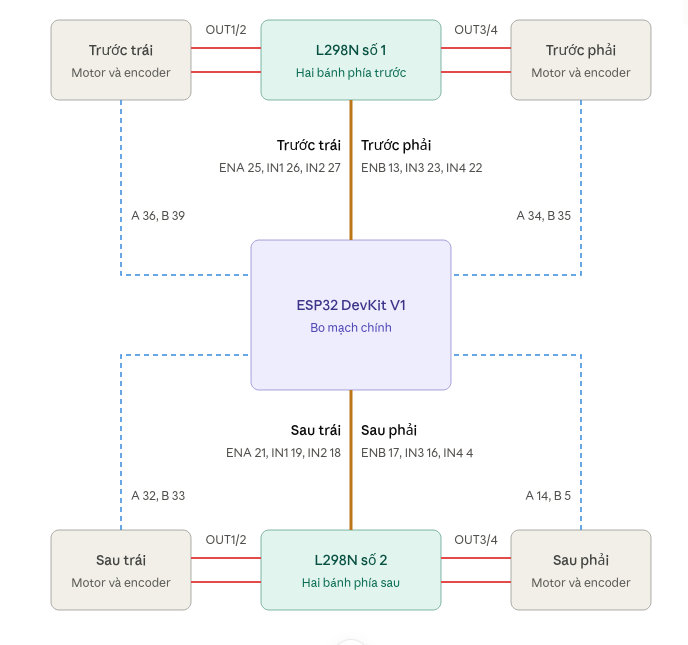
\includegraphics[width=0.85\textwidth]{pinout.png}
  \caption{Wiring of the ESP32 DevKit V1, the two L298N modules and the four GM25-370 motors with encoders (\code{docs/pinout.png}).}
  \label{fig:pinout}
\end{figure}

%====================================================================
\section{Software}
\subsection{Two-Hand Recognition}
Recognition uses geometry on the 21 MediaPipe landmarks (VIDEO mode, confidence threshold 0.6), with no additional training.

\textbf{Extended fingers.} A finger is extended when the distance from its tip to the wrist is greater than 1.15 times the distance from its middle joint (PIP) to the wrist. The ratio is dimensionless, so it does not depend on the distance to the camera or on the rotation of the hand. If only the index finger is extended, the pointing direction is computed from the base of the finger (landmark 5) to its tip (landmark 8) and divided into 8 sectors of $45^\circ$.

\textbf{Role assignment.} The image is mirrored, but MediaPipe assigns the labels Left/Right as if it were not, so the labels are inverted from the user's point of view. \code{RoleAssigner} handles this as follows:
\begin{enumerate}
  \item Two hands: roles follow the horizontal order of the wrists; the disagreement between this order and the (flipped) labels updates a score $c_k=0.95\,c_{k-1}\pm0.05$, and when $c_k<-0.6$ the label convention is flipped.
  \item One hand: the label is voted over the last 10 frames.
  \item Just went from two hands to one and the wrist moved less than 150 px: keep the previous role.
  \item Manual mode (\code{drive\_active = False}): the driving branch is locked and any hand is the interface hand.
\end{enumerate}

\textbf{Driving-gesture filter.} \code{GestureFilter} needs 4 consecutive frames (about 0.13 s) to start a motion command and 6 frames (about 0.2 s) to stop, so a single noisy frame does not make the robot jerk.

\subsection{Interface Cursor}
The dominant hand has three poses: \emph{point} (index finger) moves the cursor, \emph{click} (index plus middle) presses or drags, and \emph{idle} (anything else) hides the cursor to avoid accidental presses. A pose must be held for 3 frames to be accepted; if the hand is lost for more than 0.3 s the cursor is hidden and every held button is released.

The index fingertip position is smoothed with a One-Euro filter ($f_{\min}=1$ Hz, $\beta=8$ in normalized coordinates); the cut-off $f_c=f_{\min}+\beta|\dot x|$ is low when the hand is still and increases with hand speed.

\textbf{Action-point anchor (\code{FREEZE\_BACK}).} Raising the middle finger to click can pull the index fingertip away from the button being aimed at (measured on real hands in Section~\ref{sec:verify}). When the pose changes from point to click at time $t$, the system takes the latest filtered position that is at least 0.2 s old as the origin and keeps the compensating offset for the whole click:
\begin{equation}
(x_a,y_a)=(x_j,y_j),\ j=\arg\max\{t_j:\ t-t_j\ge0.2\},\qquad
(a_x,a_y)=\mathrm{clamp}\bigl(x+x_a-x(t),\ y+y_a-y(t)\bigr).
\end{equation}
The displayed cursor still follows the fingertip, so dragging stays smooth. After release the offset decays exponentially with a time constant of 0.15 s (\code{OFFSET\_TAU}). Sliders use relative grabbing: hold still to grab, move the finger to drag, hold still again to release. Fig.~\ref{fig:click} illustrates this on a simulated hand.

\begin{figure}[H]
  \centering
  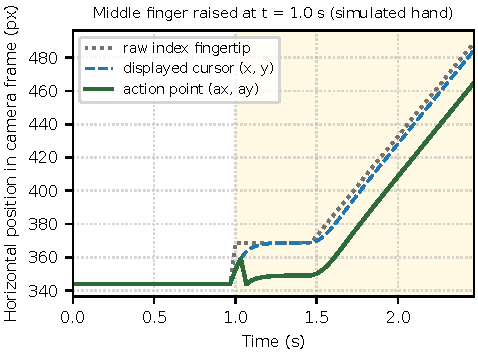
\includegraphics[width=0.6\textwidth]{fig_click_en.pdf}
  \caption{Action-point anchor on a simulated hand (using the actual \code{Cursor} class). Raising the middle finger at $t=1.0$ s shifts the fingertip by 25 px.}
  \label{fig:click}
\end{figure}

\textbf{Mapping near the frame edge.}\label{sec:edge} Hand detection fails when the hand is cut by the frame border, so a cursor that coincides with the fingertip cannot reach the corners of the screen. Let $d=f-\tfrac12$ be the fingertip position in the frame ($f\in[0,1]$, per axis), $a=0.10$ the half width of the central zone and $b=0.44$ the distance at which the cursor should reach the screen edge. With $k=(0.5-b)/(b-a)^2$ the stretched coordinate is $s=\tfrac12+\operatorname{sgn}(d)\min\{\tfrac12,\ |d|+k(|d|-a)^2\}$ for $|d|>a$ and $s=f$ otherwise, which keeps the cursor on the fingertip in the middle, grows the lead smoothly without a kink (peak gain $1.35$) and reaches the screen edge when the fingertip is $6\,\%$ of the frame from the border. If the hand is lost while the fingertip is within $12\,\%$ of the border, the cursor and pose are held for $1.0\,\mathrm{s}$ instead of $0.3\,\mathrm{s}$. A first version, with a linear ramp starting at $|d|=0.30$ and peak gain $1.67$, made the cursor visibly run ahead of the fingertip and was replaced by this one. Nine of the $55$ automatic checks cover this mapping.

\subsection{Communication Protocol}
For continuous 20 Hz motion commands only the latest value is useful, so UDP was chosen: a dropped packet is ignored and replaced 50 ms later, whereas TCP would hold back newer packets behind a lost one. On the ESP32 the Wi-Fi modem sleep is disabled (\code{WiFi.setSleep(false)}) to reduce latency. The frame is ASCII text, easy to debug:
\begin{center}\small
\code{C <seq> <vx> <vy> <w>}\quad (laptop $\to$ ESP32), e.g. \code{C 142 0.500 -0.200 0.000}\\
\code{A <seq> <m0 d0 p0 ... m3 d3 p3>}\quad (ESP32 $\to$ laptop; target, measured, PWM of the 4 wheels)
\end{center}
\textbf{Layered safety.} (1) The ESP32 accepts commands only from the first valid sender and rejects other addresses until that sender has been silent for more than 300 ms. (2) The ESP32 returns the command $(0,0,0)$ if no new packet arrives for 300 ms. (3) The laptop sets the target velocity to 0 if no new command arrives from the selected mode for 0.4 s. (4) The \code{ramp()} limiter has a maximum acceleration of 2.0/s and a maximum deceleration of 4.0/s, and forces the velocity through 0 before it changes sign.

\subsection{Closed-Loop Control on the ESP32}\label{sec:control}
Every 10 ms (100 Hz), \code{firmware/src/wheel.h} reads the counts from the hardware PCNT counter in $\times4$ quadrature decoding mode (8112 counts/wheel revolution = 26 counts/channel $\times4\times78$) with a 12.5 $\mu$s hardware glitch filter, so counting does not use CPU time. Because a single count in 10 ms already equals 2.3\,\% of full speed, the measured speed is low-pass filtered with a first-order filter:
\begin{equation}
\omega_i(k)=0.7\,\omega_i(k-1)+0.3\,\frac{c_i(k)}{4300},
\end{equation}
with $c_i$ the counts per second. The target $r_i$ of each wheel moves toward the commanded value with a maximum slope of 4.0/s. The control law (Fig.~\ref{fig:ctrl}) is:
\begin{align}
u^{\mathrm{ff}}_i&=\operatorname{sgn}(r_i)\bigl(a_i+b_i|r_i|\bigr), \quad e_i=r_i-\omega_i,\\
I_i&\leftarrow I_i+K_i e_i\,\Delta t\quad\text{only when not ramping and not saturated},\\
u_i&=\mathrm{clamp}\bigl(u^{\mathrm{ff}}_i+K_p e_i+I_i,\,-1,\,1\bigr),\qquad K_p=0.8,\ K_i=6.0.
\end{align}
The L298N plus GM25-370 system is strongly non-linear: the PWM threshold at which a wheel starts to turn differs between wheels (5.5\,\% to 14.8\,\%, a factor of 2.7) and about 44\,\% PWM already gives 80\,\% of the no-load speed. The coefficients $a_i$, $b_i$ (Table~\ref{tab:ff}) are least-squares lines fitted to steady-state points measured with the wheels lifted, using \code{firmware/tools/motor\_test.cpp}; the maximum fitting deviation is 0.045 PWM. The feed-forward term supplies approximately the right PWM immediately, and the PI term only compensates the remainder (especially the real load on the floor). Freezing the integral while ramping or saturated avoids accumulating error while the target is still moving (windup). There is no comparison with a plain PID or open loop on the same trajectories, so the improvement has not been quantified.

\textbf{Jam protection.} If the PWM is at least 0.95 while the measured speed stays below 0.05 for more than 0.7 s (\code{STALL\_SECONDS}), that wheel is switched off and an error is reported over Serial until the command returns to 0.

\begin{figure}[H]
  \centering
  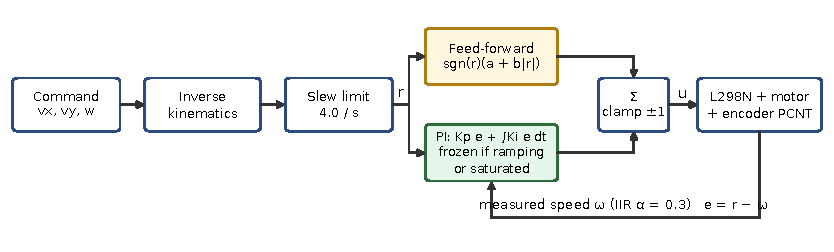
\includegraphics[width=\textwidth]{fig_ctrl_en.pdf}
  \caption{Speed controller of one wheel (100 Hz).}
  \label{fig:ctrl}
\end{figure}

\begin{table}[H]
\caption{Measured feed-forward parameters and mean tracking error on the floor (\% of full speed).}
\label{tab:ff}
\centering\small
\begin{tabular}{lccccc}
\toprule
Wheel & $a_i$ (\code{FF\_OFFSET}) & $b_i$ (\code{FF\_SLOPE}) & Manual v1 & Gesture v1 & Two-hand v2 \\
\midrule
tt & 0.076 & 0.470 & 1.8 & 1.9 & 2.5 \\
tp & 0.148 & 0.594 & 3.2 & 2.5 & 2.6 \\
st & 0.055 & 0.453 & 1.7 & 1.6 & 2.3 \\
sp & 0.060 & 0.464 & 1.5 & 1.7 & 2.5 \\
\bottomrule
\end{tabular}
\end{table}

\subsection{Web Interface}
The dashboard (FastAPI, WebSocket, single page with no scrolling) has two modes: Manual (virtual joystick, rotation buttons, arrow keys or W A S D, Q E, Space) and Hand Gesture. Every button, slider and joystick can be operated with the dominant-hand cursor; the gesture mapping is in Table~\ref{tab:gest}. Fig.~\ref{fig:ui} was captured from the running application with no camera attached.
\begin{figure}[H]
  \centering
  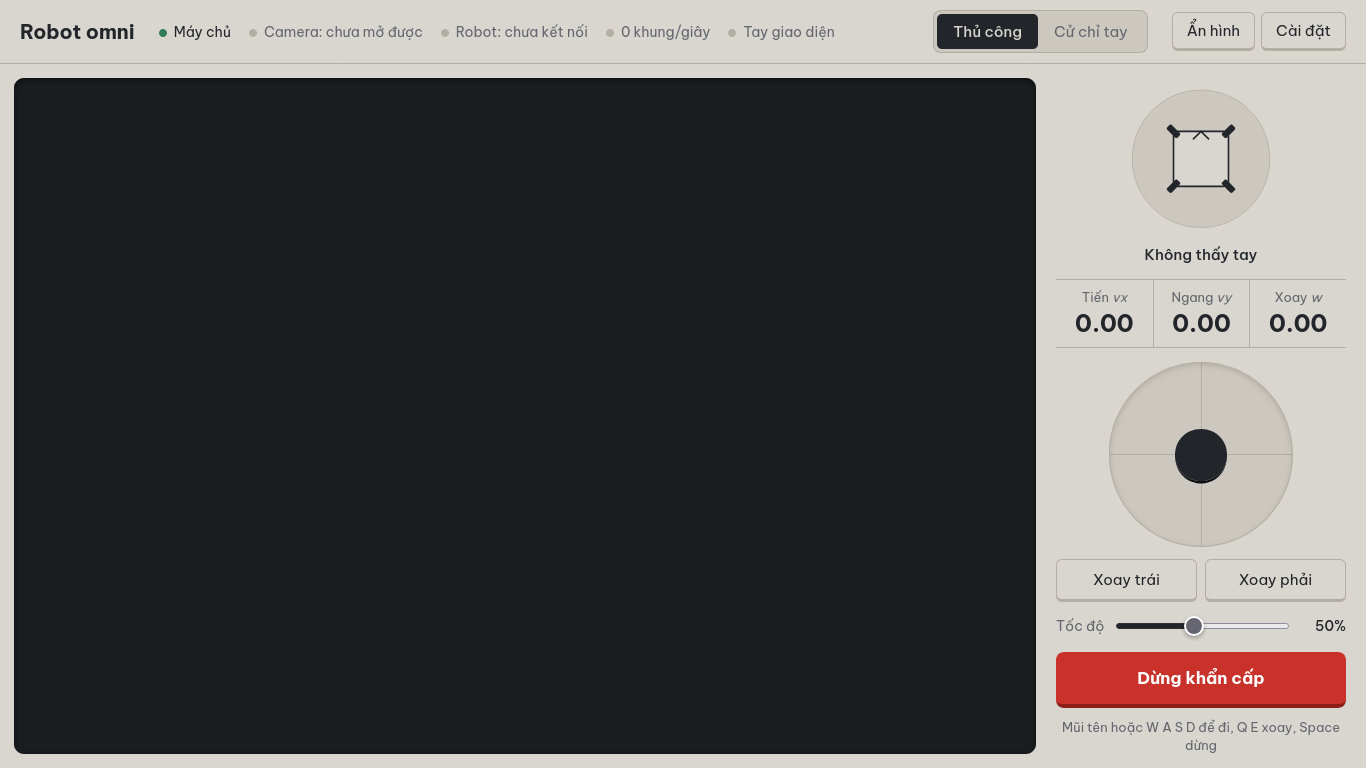
\includegraphics[width=0.9\textwidth]{dashboard.png}
  \caption{The dashboard in Manual mode.}
  \label{fig:ui}
\end{figure}

\begin{table}[H]
\caption{Gesture mapping ($s\in[0.1,1]$ is the speed factor).}
\label{tab:gest}
\centering\small
\begin{tabular}{p{2.4cm}p{3.6cm}p{5.6cm}}
\toprule
Hand & Gesture & Effect \\
\midrule
Non-dominant & fist, open palm, hand lost & Stop: $(0,0,0)$ \\
Non-dominant & point up / down & Forward $(+s,0,0)$ / backward $(-s,0,0)$ \\
Non-dominant & point left / right & Left $(0,+s,0)$ / right $(0,-s,0)$ \\
Non-dominant & point diagonally & Diagonal $(\pm0.707s,\pm0.707s,0)$ \\
Non-dominant & V sign left / right & Rotate left $(0,0,+s)$ / right $(0,0,-s)$ \\
Dominant & point & Move the cursor; hold still 0.8 s to click or grab a slider \\
Dominant & point plus middle & Quick click; hold and move to drag \\
Dominant & other, hand lost & Hide the cursor, release every held button \\
\bottomrule
\end{tabular}
\end{table}

%====================================================================
\section{Verification and Data Analysis}\label{sec:verify}
\subsection{Automatic Tests}
\begin{itemize}
  \item \code{tests/test\_hands\_logic.py}: 55 checks on synthetic hands (including the edge mapping of the cursor) built by mathematics, covering gesture classification, interface pose, role assignment with inverted labels, self-calibration, the One-Euro filter and the action-point anchor. Result: 55/55 pass.
  \item \code{tests/handcursor\_test.html}: 49 checks in a browser for dwell click, two-finger click, relative slider grab, joystick drag, hold buttons, automatic release on hand loss and the info card. Run with headless Chrome ($1280\times900$ window) on 12 November 2026: 49/49 pass. A window that is too short (below about 500 px) makes one cursor-position check fail falsely because the cursor is clamped to the window edge.
\end{itemize}
The automatic checks use a simulated hand, so their numbers only describe the algorithm on ideal data. With 2 px noise (200 seeded runs) the standard deviation of the cursor fell from 0.0047 to 0.0016 (65.5\,\% reduction). With the index fingertip displaced by $(25,-15)$ px when the middle finger is raised, the action point shifted by 0.0126 (normalized units) against 0.0770 for the fingertip, a reduction of 83.6\,\%; the residual is 4.6 px out of 29.2 px. Because the click pose is accepted only after 3 frames, the action point can briefly deviate by up to 15.6 px (about 0.1 s) before compensation.

\textbf{Measurement on a real hand.} We ran \code{tests/real\_hand\_eval.py} (the same \code{Cursor} class, real camera images, one test subject); data in \code{docs/data/v2/real\_hand\_click\_still.csv} and \code{real\_hand\_jitter.json}. \emph{Hold-still jitter:} with the index finger held still for 8 seconds (209 frames), the standard deviation of the raw fingertip was 2.26 px and that of the filtered cursor 2.14 px, a reduction of only 5\,\% (65.5\,\% in simulation). The simulation used independent noise, whereas real tremor and landmark drift are probably slow and correlated, so a low-pass filter tuned for responsiveness does not remove them; we have not tested this hypothesis. \emph{Click shift:} the subject pointed at a spot and held still (the script waited until the fingertip stayed within 3 px for 1 second and rejected trials where the hand was still drifting), then raised the middle finger, 12 times. The index fingertip moved by a median of 1.65 px (1.1--5.7), far less than the 29.2 px assumed in the simulation. The anchored action point moved by a median of 4.15 px (2.0--12.0), more than the fingertip in 11 of 12 trials (Fig.~\ref{fig:real}); the displayed cursor moved 1.9 px. So for this subject, with the finger held still, the 0.2 s look-back added about 2.5 px instead of compensating a shift. A possible reason is that the real shift is of the same size as the hand tremor, so the anchor samples the tremor instead of correcting a systematic jump. An earlier run in which the subject did not keep the finger still gave a median fingertip shift of 6.8 px and is not used. These are 12 trials from one person; the click hit rate was not measured, and the dwell radius (30 px) and the button sizes are larger than these deviations, so the practical effect on pressing is probably small but unverified. For other users or hand shapes with a stronger fingertip jump, the anchor may still help.

\begin{figure}[H]
  \centering
  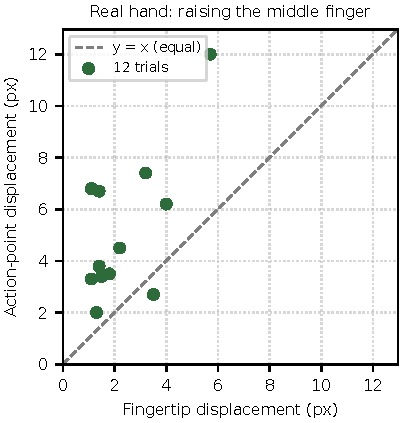
\includegraphics[width=0.45\textwidth]{fig_real_en.pdf}
  \caption{Real hand, 12 trials with the finger held still: displacement of the action point against that of the raw fingertip when the middle finger is raised. Points above the dashed line mean the action point moved more than the fingertip.}
  \label{fig:real}
\end{figure}

\subsection{Real Run Data}
Three floor runs, logged at 20 Hz, were analyzed with \code{tests/analyze\_drive\_log.py}; the data are in \code{docs/data/v1/} and \code{docs/data/v2/} (Table~\ref{tab:data}). Rows recorded while the motor supply was off (53 rows in the manual run) are excluded.

\begin{table}[H]
\caption{The logged runs.}
\label{tab:data}
\centering\small
\begin{tabular}{>{\raggedright\arraybackslash}p{5.2cm}rr>{\raggedleft\arraybackslash}p{3.4cm}}
\toprule
Run (file) & Rows & Duration (s) & RTT median / P95 / max (ms) \\
\midrule
Manual v1 (\code{drive\_manual.csv}) & 3240 & 1512 & 7.8 / 22.5 / 97 \\
Gesture v1 (\code{drive\_gesture.csv}) & 4820 & 247 & 8.1 / 26.1 / 101 \\
Two-hand v2 (\code{drive\_twohand.csv}) & 5020 & 266 & 6.6 / 16.1 / 909 \\
\midrule
Total & 13080 & 2026 & -- \\
\bottomrule
\end{tabular}
\end{table}
The manual run contains 389 rows in gesture mode. The maximum RTT in the v2 run was 909 ms, far above the 300 ms limit of the ESP32, so the robot would stop in such a case.

\textbf{Latency.} From the moment a motion gesture is recorded until the most loaded wheel reaches 50\,\% of its new target: median 260 ms (204--359 ms, 38 events, v1) and 257 ms (203--309 ms, 26 events, v2). These figures include the deliberate acceleration limit and are therefore not the smallest achievable latency.

\textbf{Gesture stability.} Among 120 gesture changes (v1), 7 segments lasted less than 0.3 s (5.8\,\%); among 76 (v2), 5 segments (6.6\,\%). We did not annotate whether these short segments were unintended actions.

\textbf{Speed tracking.} Only counted when the command was constant for 0.3 s and at least 0.1 in magnitude. The mean error is 1.5--3.2\,\% (Table~\ref{tab:ff}, Fig.~\ref{fig:wheel}). The 95th percentile is 4.4--4.8\,\% in the v1 gesture run but 6.1--7.4\,\% in the v2 two-hand run, so the 5\,\% target is met by the mean but not by the 95th percentile in the v2 run. The mean PWM of the tp wheel is the highest (0.48--0.49 against 0.36--0.44 for the other wheels), consistent with its largest dead zone.

\begin{figure}[H]
  \centering
  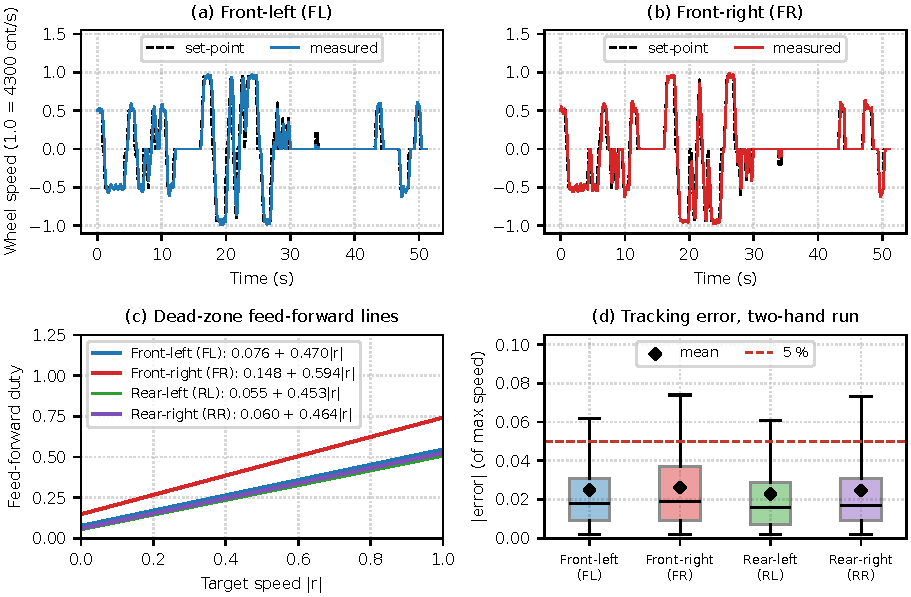
\includegraphics[width=\textwidth]{fig_wheel_en.pdf}
  \caption{Wheel speed control, two-hand run. (a), (b): set-point and measured speed of two wheels over 50 s; (c): feed-forward lines; (d): distribution of the steady-state error (whiskers: 5th--95th percentile; diamond: mean; dashed line: 5\,\%).}
  \label{fig:wheel}
\end{figure}

\textbf{Body motion.} Table~\ref{tab:odo} compares the command with the velocity computed from the encoders using (\ref{eq:fk}); Fig.~\ref{fig:rtt} shows the RTT distribution and the velocity magnitudes. The deviation on the main axis is below 0.6\,\% for translation and 2.4--2.5\,\% for rotation, and unintended motion on the other axes is at most 0.004. These are velocities inferred from the encoders and do not include wheel slip on the floor, so they are not true position errors.

\begin{table}[H]
\caption{Command versus forward kinematics. The first six rows are from the v1 gesture run, the two diagonal rows from the v2 run.}
\label{tab:odo}
\centering\footnotesize\setlength{\tabcolsep}{3pt}
\begin{tabular}{lrccrr}
\toprule
Motion & Samples & Command $(v_x,v_y,\omega)$ & From encoders & Main-axis dev. & Other axis \\
\midrule
Forward & 543 & (+0.472; 0; 0) & (+0.474; +0.001; +0.002) & +0.6\,\% & 0.002 \\
Backward & 360 & (-0.510; 0; 0) & (-0.510; -0.001; -0.001) & -0.1\,\% & 0.001 \\
Left & 96 & (0; +0.480; 0) & (+0.004; +0.482; +0.002) & +0.4\,\% & 0.004 \\
Right & 73 & (0; -0.480; 0) & (-0.003; -0.479; 0) & -0.2\,\% & 0.003 \\
Rotate left & 238 & (0; 0; +0.435) & (+0.003; +0.001; +0.446) & +2.5\,\% & 0.003 \\
Rotate right & 230 & (0; 0; -0.442) & (-0.001; 0; -0.453) & +2.4\,\% & 0.001 \\
Forward-left (v2) & 98 & (+0.308; +0.245; 0) & (+0.316; +0.256; +0.001) & -- & -- \\
Forward-right (v2) & 71 & (+0.313; -0.237; 0) & (+0.316; -0.243; -0.002) & -- & -- \\
\bottomrule
\end{tabular}
\end{table}

\begin{figure}[H]
  \centering
  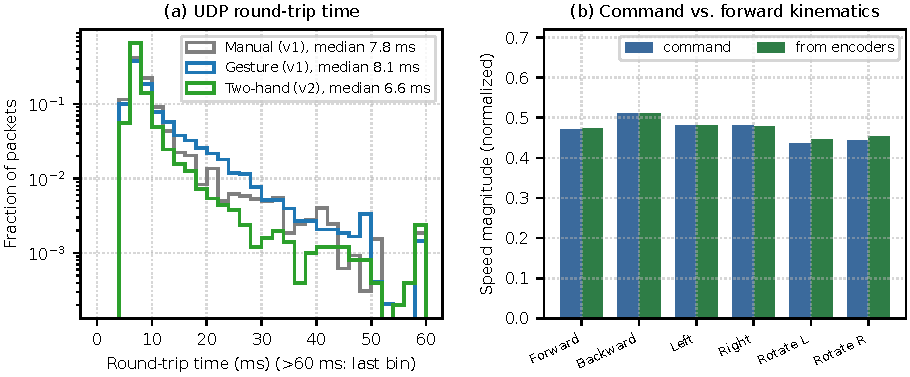
\includegraphics[width=\textwidth]{fig_rtt_odo_en.pdf}
  \caption{(a) RTT distribution of the three runs (log scale, values above 60 ms fall into the last bin). (b) Magnitude of the commanded velocity and of the velocity from the encoders for the six basic motions.}
  \label{fig:rtt}
\end{figure}

\subsection{Second Session: Vision Loop with Hands, End-to-End Latency and the Cursor near the Frame Edge}
After the runs above we recorded four more server sessions with the per-run logger (\texttt{web/runlog.py}): one log row per camera frame, plus the 20\,Hz drive log when the robot was connected (data in \texttt{docs/data/v2/session2/}, table~\ref{tab:sess2}). Sessions A and B ran the code from before the changes described below (MJPG $640\times480$ capture, cursor mapped 1:1 to the fingertip); sessions C and D ran after the capture was raised to $1280\times720$ (hand detection still on a $640$-px-wide copy) and after the cursor was made to move faster than the fingertip near the frame edge (C with a piecewise-linear mapping, D with the smooth mapping of Section~\ref{sec:edge}). A and B had the robot connected; C and D tested the cursor only. A is the first run after a wheel fault was repaired, and D was still running when its log was copied, so D is a snapshot. One operator took part in all four sessions, and the sessions differ in what the operator did, in the number of open browser tabs and in duration, so they are not a controlled comparison.

\begin{table}[H]
\caption{Server sessions recorded with the per-run logger. Mean hand-landmark inference time (ms) is split by the number of hands in the frame; fps is the number of AI frames per second over the whole session.}
\label{tab:sess2}
\centering
\footnotesize
\setlength{\tabcolsep}{3pt}
\begin{tabular}{llcrrrrr}
\toprule
Sess. & Camera & Cursor & Time (s) & fps & 0 hand & 1 hand & 2 hands \\
\midrule
A & 640$\times$480 & 1:1 & 186 & 25.5 & 27.7 & 45.5 & 43.3 \\
B & 640$\times$480 & 1:1 & 76 & 21.9 & 31.3 & 50.1\textsuperscript{a} & 47.5 \\
C & 1280$\times$720 & piecewise & 363 & 18.0 & 30.7 & 55.5 & 48.3 \\
D & 1280$\times$720 & smooth & 214 & 21.9 & 28.9 & 52.4 & 47.2 \\
\bottomrule
\multicolumn{8}{l}{\footnotesize\textsuperscript{a}Only 46 frames with exactly one hand.}\\
\end{tabular}
\end{table}

\emph{Vision loop with hands.} With no hand in view, inference averaged 27.7--31.3 ms; with one hand 45.5--55.5 ms and with two hands 43.3--48.3 ms (Fig.~\ref{fig:sess2}a). The frame rate over a whole session was 18.0--25.5 fps, below the 25 fps target and below the 29.9 fps of the isolated benchmark above, which measured capture and detection alone with no hand; the server also encodes and streams every frame and runs the control loop, and the cause of the difference was not isolated. Frames with one hand were not cheaper than frames with two (a possible reason, that the detector keeps searching for the missing second hand, was not tested). Raising the capture to $1280\times720$ did not change the no-hand cost (27.7--31.3 ms in all four sessions); with one hand the mean was higher in C and D than in A (55.5 and 52.4 against 45.5 ms), but the sessions are not comparable enough to attribute this to the resolution.

\begin{figure}[H]
  \centering
  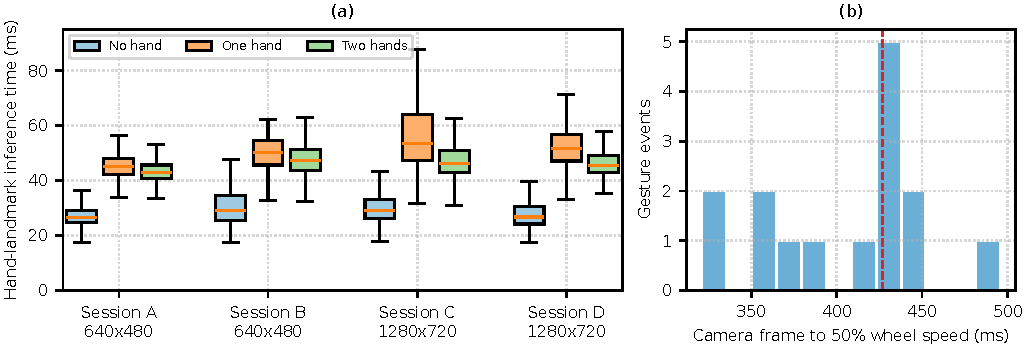
\includegraphics[width=\textwidth]{fig_sess2_en.pdf}
  \caption{(a) Hand-landmark inference time per session and number of hands in view (boxes: quartiles; whiskers without outliers). (b) Delay from the camera frame in which the gesture filter confirmed a motion gesture to the moment the most loaded wheel reached 50\,\% of its new target, session A (15 events; dashed: median).}
  \label{fig:sess2}
\end{figure}

\emph{End-to-end latency (session A).} For 15 confirmed motion gestures, the median time from the camera frame in which the gesture filter fired to the moment the most loaded wheel reached 50\,\% of its new target was 427 ms (321--496 ms, Fig.~\ref{fig:sess2}b); the command left the laptop 37 ms after that frame (median). The filter itself needs $4$ consecutive frames, about three frame intervals ($120$--$140$ ms at these frame rates) before the confirming frame, which is not included. The median target magnitude was 0.81 of full speed; with the host acceleration limit of $2.0\,\mathrm{s^{-1}}$ half of that takes about $0.2\,\mathrm{s}$, so a large part of the delay is the deliberate ramp. This is longer than the $257$--$260\,\mathrm{ms}$ reported in Section~5.2, which started from the gesture value written in the drive log instead of the camera frame (about 37 ms later) and used targets of other sizes; the 15 events here are too few and too uniform to separate these causes. Session B contains a single event (319 ms, target 0.5).

\emph{Wheel tracking and link.} With the same rule as in Section~5.2, the mean error was 1.3\,\% (manual) and 1.5\,\% (gesture) of full scale in A, and 0.9\,\% in B (gesture only; $12$ manual samples are too few to report), with $95$th percentiles of 4.3, 5.0 and 4.2\,\%. In A the duty was at the $0.95$ ceiling in 8.0\,\% of the manual and 3.8\,\% of the gesture samples, against 0.0\,\% in B: at the higher speeds of A the controller ran out of voltage headroom, so the commanded speed could not be reached, which can distort diagonal motion if the wheels saturate unequally (not measured). The UDP round trip had a median of 6.4 and 7.9 ms (95th percentile 23.9 and 17.3 ms; maximum 104 and 47 ms), consistent with the earlier runs.

\emph{Cursor near the frame edge.} The mapping of Section~\ref{sec:edge} was introduced after the operator reported that the UI hand was lost whenever the fingertip had to reach the frame border to hit the speed slider in the screen corner, and then that the cursor ran ahead of the fingertip when the stretch started abruptly. The logs give an indirect view only, because they do not store the raw fingertip position: the share of UI-hand frames with the cursor within $2\,\%$ of a screen edge was 2.3\,\% in A and 1.4\,\% in B (1:1 mapping), and 8.2\,\% in C and 4.6\,\% in D (stretched); the number of UI-hand segments longer than $0.3\,\mathrm{s}$ that ended with the cursor at an edge, a sign of losing the hand there, was 1 of 6 in A, 1 of 3 in B, 0 of 15 in C and 1 of 9 in D. The operator also needed the corner more in C and D because the task was to reach it, so these numbers show that the cursor reaches the screen edge with the stretched mapping, not that hand loss was reduced; the counts are small. The lead of the cursor over the fingertip near the edge (up to $6\,\%$ of the frame width by construction) was not measured against the fingertip position and rests on the operator's report.

%====================================================================
\section{Limitations and Reproduction}
\textbf{Limitations.} The data come from one robot, one floor and one operator. There is no user study. The real-hand cursor measurements (jitter, click shift) come from one person and 12 clicks, and the click hit rate was not measured; the FREEZE\_BACK anchor did not give better results in these measurements. There is no comparison of the controller with a plain PID or open loop. The end-to-end latency was measured in one session (15 events), and the effect of the edge mapping on hand loss was not measured against the true fingertip position. The robot has no obstacle sensing.

\textbf{Reproducing the data and figures.} From the project root:
\begin{center}\small
\code{.venv/bin/python reports/make\_figures.py}\quad (generates the figures and \code{reports/figures/stats.json})\\
\code{python tests/analyze\_drive\_log.py docs/data/v2/drive\_twohand.csv}\\
\code{.venv/bin/python reports/session2.py}\quad (second session: \code{stats\_session2.json} and figure)\\
\code{python tests/analyze\_run.py logs/ai\_<time>.csv logs/drive\_<time>.csv}\\
\code{python tests/test\_hands\_logic.py}\quad \code{python tests/camera\_fps\_test.py}
\end{center}
\end{document}
